\chapter{Background}
\label{chap:Background}

% NOTE: (aver) Explain important topics for the reader to understand

\section{Distributed Ledger Technology} % (fold)
\label{sec:Distributed Ledger Technology}

Distributed Ledger Technology, DLT, refers to the technology of the decentralized database, which provides control over
the development of data between various entities through a peer-2-peer network. In order to achieve synchronicity across
nodes of the network, consensus algorithms are used.

% TODO: (aver) Explain DLT
% also the difference between BC vs DLT.

\subsection{Blockchains} % (fold)
\label{sub:Blockchains}

% subsection Blockchains (end)

\subsection{Smart Contract} % (fold)
\label{sec:Smart Contract}

% subsection Smart Contract (end)
% section Distributed Ledger Technology (end)

\section{Sovereignty} % (fold)
\label{sec:Sovereignty}

Self-sovereign Identity is compromised of 3 main pillar, blockchains, DIDs, and VCs.

% section Sovereignty (end)


\section{Manufacture Usage Description} % (fold)
\label{sec:Manufacture Usage Description}

MUD has been developed by the International Engineering Task Force, IETF, with following goals and intents in mind:
\cite{rfc8520-mud}
\begin{itemize}
	\item Substantially reduce the threat surface on a device to those communications intended by the manufacturer.
	\item Provide a means to scale network policies to the ever-increasing number of types of devices in the network.
	\item Provide a means to address at least some vulnerabilities in a way that is faster than the time it might
	      take to update systems. This will be particularly true for systems that are no longer supported.
	\item Keep the cost of implementation of such a system to the bare minimum.
	\item Provide a means of extensibility for manufacturers to express other device capabilities or requirements.
\end{itemize}

MUD does not entail address network authorization of general purpose computers, it simply creates a suggestion than can
be followed.
The architecture of Devices using MUD can be seen in Figure~\ref{fig:NIST MUD Reference Architecture}, which is the
reference architecture by NIST \cite{dodson2021securing} but it can be found in similar fashion inside the RFC
specification.

\begin{figure}
	\begin{center}
		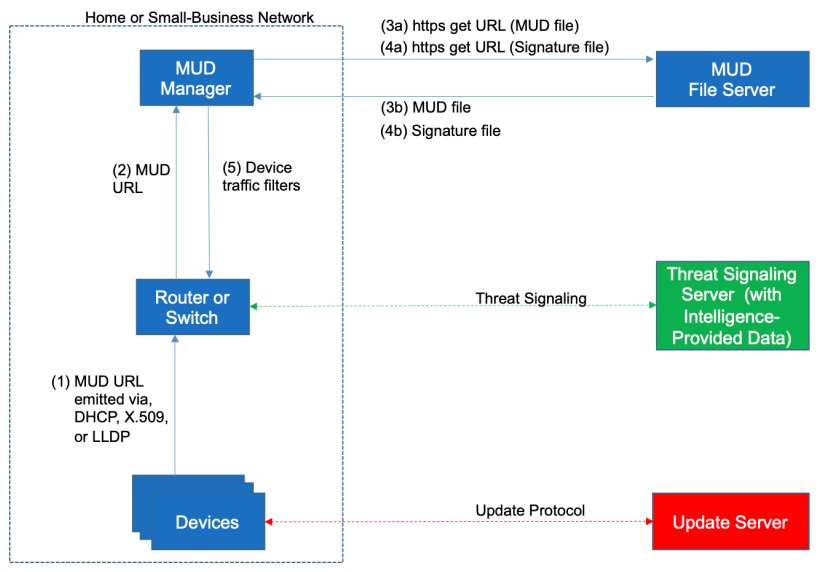
\includegraphics[width=0.95\textwidth]{figures/nist-mud-arch.png}
	\end{center}
	\caption{NIST MUD Reference Architecture}
	\label{fig:NIST MUD Reference Architecture}
\end{figure}
% section Manufacture Usage Description (end)

\section{Physical Unclonable Function} % (fold)
\label{sec:Physical Unclonable Function}

In order to be able to track IoT nodes in a blockchain, they need to be uniquely identifiable, in our case even in a
distributed manner, using e.g., Distributed Identifiers, DIDs.
Common practices are based on placing a cryptographic key into a nonvolatile electrically erasable programmable
read-only memory (EEPROM) or battery-backed static random-access memory (SRAM) and use hardware cryptographic operations
such as digital signatures or encryption, which is all expensive in design and power consumption. \cite{herder2014physical}

PUFs are unpredictable and uncontrollable, therefore making it unclonable and an ideal security vector. They are
dependent on random physical factors introduced during manufacturing, e.g., inequalities of SRAM cells, although factors
such as the altering of the physical components, voltage and temperature need to be taken into account. \cite{vinagrero2023sram}
For reasons of simplicity and because it is not the main focus of this thesis, we will neglect this aspect.
% TODO: Specify assumptions in another paragraph

By implementing the Challenge-Response Pair, CRP, is used to evaluate the microstructure, whereas a physical challenge
makes the device react, the response, in an unpredictable, but repeatable way.
In order to turn this 'silicon key' into a cryptographic root key, processing algorithms need to be applied, that ensure
that the distribution of 0s and 1s are uniform. \cite{herder2014physical}

\subsubsection{SRAM-Based PUF Readouts} % (fold)
\label{sec:SRAM-Based PUF Readouts}

Methods of creating identifiers that are unique to devices exist, such as SRAM-Based Physical Unclonable Function, PUF,
readouts. Therein PUFs are among the most cost-effective security primitives to establish hardware trust.
\cite{holcomb2007initial}

Even though the evaluation process of the characterization of guarantee over lifetime and differing operating conditions
are still subject to research following metrics have become widespread: \textit{reliability}, the variation of bit-wise
startup patterns; \textit{uniformity}, i.e., the repeatability and reproducibility on a given device after any amount of
restarts; \textit{uniqueness}, the probability of other devices with same signatures; \textit{bit-aliasing}, the
probability of specific bit position of the signature to be biased towards 0 or 1. \cite{vinagrero2023sram}
% subsubsection SRAM-Based PUF Readouts (end)


% TODO: (aver) challenges, vulnerabilities

% section Physical Unclonable Function (end)

\section{Over the Air IoT updating} % (fold)
\label{sec:Over the Air  IoT updating}
In order to stray away from the classic client-server architecture for updating devices, which demonstrate a single
point of failure, we will discuss other decentralized methods to achieve Over the Air, OTA, updates for IoT devices.

\subsection{Distributed OTA} % (fold)
\label{sub:Distributed OTA}

% subsection Distributed OTA (end)
% section Over the Air IoT updating (end)
